%
% Annual Cognitive Science Conference
% Sample LaTeX Paper -- Proceedings Format
%

% Original : Ashwin Ram (ashwin@cc.gatech.edu)       04/01/1994
% Modified : Johanna Moore (jmoore@cs.pitt.edu)      03/17/1995
% Modified : David Noelle (noelle@ucsd.edu)          03/15/1996
% Modified : Pat Langley (langley@cs.stanford.edu)   01/26/1997
% Latex2e corrections by Ramin Charles Nakisa        01/28/1997
% Modified : Tina Eliassi-Rad (eliassi@cs.wisc.edu)  01/31/1998
% Modified : Trisha Yannuzzi (trisha@ircs.upenn.edu) 12/28/1999 (in process)
% Modified : Mary Ellen Foster (M.E.Foster@ed.ac.uk) 12/11/2000
% Modified : Ken Forbus                              01/23/2004
% Modified : Eli M. Silk (esilk@pitt.edu)            05/24/2005
% Modified : Niels Taatgen (taatgen@cmu.edu)         10/24/2006
% Modified : David Noelle (dnoelle@ucmerced.edu)     11/19/2014
% Modified : Roger Levy (rplevy@mit.edu)     12/31/2018



%% Change "letterpaper" in the following line to "a4paper" if you must.

\documentclass[10pt,letterpaper]{article}

\usepackage{cogsci}

\cogscifinalcopy % Uncomment this line for the final submission

\usepackage{graphicx}
\usepackage{pslatex}
\usepackage{apacite}
\usepackage{float} % Roger Levy added this and changed figure/table
                   % placement to [H] for conformity to Word template,
                   % though floating tables and figures to top is
                   % still generally recommended!

%\usepackage[none]{hyphenat} % Sometimes it can be useful to turn off
%hyphenation for purposes such as spell checking of the resulting
%PDF.  Uncomment this block to turn off hyphenation.


%\setlength\titlebox{4.5cm}
% You can expand the titlebox if you need extra space
% to show all the authors. Please do not make the titlebox
% smaller than 4.5cm (the original size).
%%If you do, we reserve the right to require you to change it back in
%%the camera-ready version, which could interfere with the timely
%%appearance of your paper in the Proceedings.



\title{Controlling the retrieval of general vs specific semantic knowledge in the instance theory of semantic memory}

\author{{\large \bf Matthew J. C. Crump (mcrump@brooklyn.cuny.edu)} \\
  Department of Psychology, 2900 Bedford Ave \\
  Brooklyn, NY 1120 USA
  \AND {\large \bf Randall K. Jamieson (randy.jamieson@umanitoba.ca)} \\
  Department of Psychology, 190 Dysart Rd \\
  Winnipeg, MB R3T 2N2 Canada}


\begin{document}

\maketitle


\begin{abstract}
Distributional models of semantic cognition produce word-embeddings sensitive to how words co-occur in local contexts in natural language. Word-embedding similarity space can be compromised by high frequency words, but strategies for managing base rates of word occurrence are usually not cognitively plausible. In a series of simulations, we show that an instance based distributional model \cite<ITS, >{jamiesonInstanceTheorySemantic2018a} can take advantage of learning and memory operations to control how base rate information is integrated into word-embeddings. We suggest these cognitive processing assumptions may allow people to control production of general versus specific semantic knowledge.

\textbf{Keywords:}
distributional semantics; negative information; instance theory; surprise-driven learning; retrieval
\end{abstract}


\section{Introduction}\label{introduction}

Distributional models of semantics produce word embeddings sensitive to word co-occurrence structure in natural text. Word embeddings are more similar between words appearing in similar than different local contexts (sentences, paragraphs). The quality of word embeddings depends on their use. For applied purposes, word-embeddings could be used to train a classifier (e.g., for sentiment analysis) and quality assessed by classifier accuracy. For theoretical purposes, distributional models of semantic cognition are evaluated by fits to human performance in semantic tasks. Word embedding quality also depends on base rates of word occurrence. High frequency words can dominate semantic vectors, causing embeddings to become more similar and less indicative of nuanced meaning. Standard approaches to managing base rate information have questionable cognitive plausibility. The present work merges assumptions from two memory models, the instance theory of semantics \cite<ITS,>{jamiesonInstanceTheorySemantic2018a} and the instance theory of associative learning \cite<MINERVA-AL,>{jamiesonInstanceTheoryAssociative2012}, to deliver a cognitively plausible means of managing base rate information for constructing veridical word embeddings.

Common base rate management strategies are stop word exclusion, transformation, and negative sub-sampling. Stop word exclusion is arbitrary and fails to account for included word base rates. Early models like LSA \cite{landauerSolutionPlatoProblem1997} used transformation. Word frequencies were log transformed and divided by their entropy across document contexts. The log transform compresses frequency counts, and the division by entropy weights words by the specificity of their occurrence in local contexts. Here, context-ubiquitous high-frequency words (high entropy) are weighted less strongly than context-specific words (low entropy). Neural network models like word2vec \cite{mikolovDistributedRepresentationsWords2013} use a process of sub-sampling adversarial examples during training. Here, network weights are modified by prediction error from positive and negative examples; and, negative examples are chosen randomly as a function of word frequency. Importantly, word2vec produces high-quality word embeddings that can explain more variance in human semantic judgments than other models \cite{manderaExplainingHumanPerformance2017a}, and these improvements have been attributed to the sub-sampling procedure. Relatedly, \citeauthor{johnsRoleNegativeInformation2019} \citeyear{johnsRoleNegativeInformation2019} created analytic transforms mimicking the base rate management effects of sub-sampling negative information that appear to improve the quality of word-embeddings in general.

We are optimistic that distributional models hold insights for semantic cognition, but we question the cognitive plausibility of common strategies for managing base rate information. It is unlikely that people ignore stop words, unclear how people would weight word frequency knowledge by information theoretic transforms (or apply singular value decomposition), and doubtful that people employ negative sub-sampling when they encounter words. In our view, a satisfactory model should detail a cognitively plausible process for managing base rates in constructing semantic knowledge. We propose a cognitive solution for the ITS model that merges theoretical insights from traditions in memory and learning.

ITS applied instance theory principles \cite{jacobyNonanalyticCognitionMemory1984} to distributional semantics by combining BEAGLE word representations \cite{jonesRepresentingWordMeaning2007} with MINERVA 2 encoding and retrieval operations \cite{hintzmanMINERVASimulationModel1984}. ITS is unique in assuming instance rather than prototype representations, which fail to capture polysemy. For example, ``bank'' could refer to a river or financial institution; but, a prototype representation averages the distinction with a single vector partway between the two meanings. By contrast, ITS encodes individual sentences as memory traces, and produces word embeddings at the time of retrieval. Retrieval is similarity driven and context-sensitive, allowing production of semantic vectors tailored to the local context (river vs. piggy) of a probe word (bank).

ITS used the cognitively questionable, but common practice, of stop word exclusion to manage base rate information. Here, we show that ITS 2 can manage base rates in cognitively meaningful ways by adopting assumptions from memory and learning theory. In doing so, ITS 2 consolidates processing assumptions across MINERVA 2 and two extensions, ITS, and MINERVA-AL \cite{jamiesonInstanceTheoryAssociative2012} which accounts for a variety of associative learning phenomena. First, we borrow the discrepancy encoding rule from MINERVA-AL, which constrains encoding to unexpected features of an experience. However, we adopted the term "weighted-expectancy subtraction" here because we show how the principle can be applied at encoding or retrieval. Second, we borrow iterative retrieval from MINERVA 2, which allows successive waves of retrieval based on internal memory responses. By simulation, we show that these encoding and retrieval operations modulate the integration of base rate information in ITS 2 semantic vectors, and subsequently determine which aspects of the semantic space ITS recovers.

As an overview we first define ITS and ITS 2. This work is in the preliminary stage of verifying the consequences of the new processing assumptions, so we conducted simulations on an artificial language with known word co-occurrence structure. This enabled a clear accounting of the aspects of the semantic space that ITS and ITS 2 recovers. We present our simulations and then discuss testing the implications in natural languages as a next step.

\subsection{ITS and ITS 2}

We define ITS and then ITS 2 modifications. Importantly, we defined a version of ITS 2 that implemented weighted expectancy subtraction (discrepancy encoding) during encoding throughout training; and a version that used a combination of weighted expectancy subtraction and iterative retrieval only during retrieval, after training was complete.

\subsubsection{Word representation}

Following BEAGLE, words are arbitrary perceptual objects with no pre-existing similarity. Each word is assigned an environment vector by randomly sampling \(n\) values from a normal distribution (\(\mu = 0\), \(\sigma = 1/n\)), where \(n\) determines the dimensionality of the vector space. Thus, all words are ortho-normal in expectation. ITS can accommodate other representational assumptions, and for convenience and didactic purposes we used one hot coding, or a simple identity matrix.

\subsubsection{Memory}

In ITS, slices of experience with words in context are represented as composite traces and stored as new row entries to a memory matrix. For example, committing a sentence to memory involves summing the environmental vectors for the words in the sentence:

\begin{equation}
M_i = c_i = \sum_{j=1}^{j=h} w_{ij}
\label{eq:memory}
\end{equation}

\(M_i\) is the memory matrix, and \(c_i\) is a sentence context. \(c_i\) is stored in a new row in \(M_I\) as a composite trace by summing the \(w_{ij}\) environment vectors for each word, from \(1\), to \(h\), in the sentence. For example, the sentence ``I like cats'' is the sum of \(w_{I} + w_{like} + w_{cats}\). The number of words inside a trace is a windowing parameter that must be larger than one word, otherwise the memory will return perceptually similar traces, rather than semantically similar ones. We note that the memory matrix becomes a document-term matrix of word frequencies when the environment vectors for words are taken from an identity matrix.

\subsubsection{Retrieval}\label{retrieval}

Word meaning is constructed at retrieval. Memory is probed with a word and returns an echo response. The echo is the sum of similarity weighted traces to the probe, and taken as the semantic vector for the probe word. Retrieval and echo construction follow MINERVA 2. First, memory \(M\) is probed with a word environment vector  \(w_i\), and the cosine similarities between \(w_i\) and all traces \(M\) are computed to produce a vector of trace activations \(a_i\):

\begin{equation}
a_i = (\frac{\sum_{j=1}^{j=n}p_j \times M_{ij}}{\sqrt{\sum_{j=1}^{j=n}p_j^2}\sqrt{\sum_{j=1}^{j=n}M_{ij}^2}})^{tau}
\label{eq:activation}
\end{equation}

where, \(a_i\) is the activation (cosine similarity to probe) of trace \(i\) in memory, \(p_j\) are the \(jth\) features of the probe, \(M_{ij}\) are the \(jth\) features of each trace \(i\) in memory, and \(n\) is the number of columns in memory setting the dimensionality of the vector space. The vector of activations is raised to a power, \({tau}\), controlling a retrieval gradient determining selectivity in the composition of the echo. The activation vector is a record of similarity between the traces and the probe spanning the range \(-1\) to \(1\), with \(a_i = 1\) when a trace is identical to the probe, \(a_i = 0\) when a trace is orthogonal to the probe, and \(a_i = -1\) when the trace is opposite the probe.

In the second step, the activated traces are summed to produce a composite memory response, called the echo. Specifically, all traces in memory are multiplied by their activations, and the echo is formed by summing the weighted traces:

\begin{equation}
e_j = \sum_{i=1}^{i=m}\sum_{j=1}^{j=n}a_i \times M_{ij}
\label{eq:echo}
\end{equation}

where, \(e_j\) is the \(jth\) feature of the echo, \(m\) is the number of traces in memory, \(a_i\) is the activation of trace \(i\), and \(M_{ij}\) are the \(jth\) values of each trace \(i\) in memory. In ITS, the echo is used as the semantic representation for the probe word.


 by probing memory with a word to generate an echo response, which is taken as the semantic vector. Words are compared for semantic similarity by comparing their respective echoes.
As a result, semantic similarity, \(r\), between two words is computed between their respective echoes using a cosine:

\begin{equation}
r(p_1,p_2) = \frac{\sum_{j=1}^{j=n}e_{1j} \times{} e_{2j}}{\sqrt{\sum_{j=1}^{j=n}e_{1j}^2}\sqrt{\sum_{j=1}^{j=n}e_{2j}^2}}
\label{eq:semanticsim}
\end{equation}

We now describe ITS 2 modifications that manage base rate information. The modifications can be implemented during encoding throughout training, or only at retrieval after training is complete. The encoding variant is more computationally expensive, as the contents of ITS 2 memory must be transformed over the course of training the model, on a trace by trace basis.

\subsection{ITS 2: weighted expectancy subtraction at encoding}

ITS 2 implements weighted expectancy subtraction during encoding in a similar manner to MINERVA-AL's discrepancy encoding rule. The difference is the subtraction between the probe and the echo is weighted by \(x\), controlling the amount of expectation to be subtracted. Weighted expectancy subtraction is applied at each step across training. For example, when a new sentence is experienced, the sentence context vector \(c_i\) is used as a probe to memory to generate an echo. The echo represents the memories' expectation for the new sentence. If the new sentence is fully expected, then the memory can reconstruct the new sentence on the basis of its existing traces. The magnitude of the echo vector contains the sum of many traces, and is generally much larger than the magnitude of the sentence context vector. As a result, before subtraction, the probe and echo vectors are normalized,

\begin{equation}
c'_j = \frac{c_j}{\max | c_{j,n} |}
\label{eq:normprobe}
\end{equation}

where, \(c_j\) is a probe vector, and the elements of \(c_j\) are divided by the largest absolute value in \(c_j\), to produce the normalized \(c'_j\). Similarly, the echo is normalized such that,

\begin{equation}
e'_j = \frac{e_j}{\max | e_{j,n} |}
\label{eq:normecho}
\end{equation}

where, \(e_j\) is an echo vector, and the elements of \(e_j\) are divided by the largest absolute value in \(e_j\), to produce the normalized \(e'_j\).

Next, the new trace encoded to memory is defined by subtraction of a weighted normalized echo from the normalized probe,

\begin{equation}
M_{ij} = c'_j  - xe'_j
\label{eq:ITS2encoding}
\end{equation}

where, \(M_{ij}\) is the new row entry in the memory matrix, and \(x\) is a weighting parameter (from 0 to 1), controlling how the proportion of the normalized echo subtracted from the normalized probe. When \(x\) is set to 0, ITS 2 becomes equivalent to ITS.

\subsection{ITS 2: weighted expectancy subtraction at retrieval}

ITS 2 can also conduct a similar operation of weighted expectancy subtraction at the time of retrieval. In this case, memory is constructed identically to ITS, except weighted expectancy subtraction occurs at retrieval through a two-step iterative retrieval process. A probe word generates an echo from memory, and the echo is submitted as an ``internal'' probe to generate a second echo. The semantic representation for the word is taken as a weighted subtraction of the normalized second echo from the normalized first echo.

The first echo \(e_1\) is generated in the usual way, but then resubmitted as a probe to construct \(e_2\) by the same equations \ref{eq:activation} and \ref{eq:echo} used to construct \(e_1\). Both \(e_1\) and \(e_2\) are normalized following equation \ref{eq:normecho}. Whereas in ITS, the semantic representation for a word is defined as \(e_1\), the semantic representation for a word with weighted expectancy subtraction at retrieval in ITS 2 is:

\begin{equation}
s_i = e'_1 - xe'_2
\label{eq:ITS2retrieval}
\end{equation}

where, \(s_i\) is the semantic representation for the \(ith\) word, and \(x\) is a weighting parameter varying from 0 to 1 controlling the amount of \(e'_2\) subtracted from \(e'_1\).

\section{Simulations}

\begin{figure*}

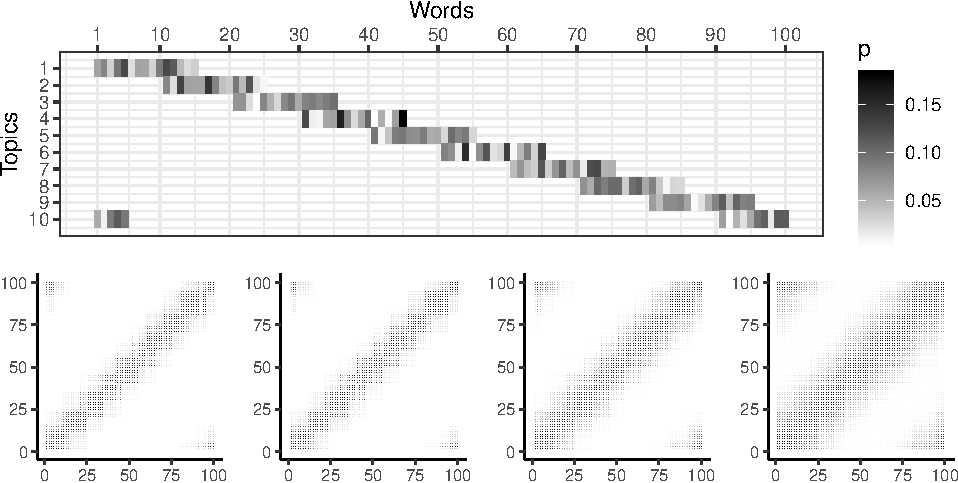
\includegraphics[width=\textwidth]{ITS_cogsci_files/figure-latex/artlang-1.pdf}

\caption{Upper: The topic-word probability matrix defining the artificial language. Darker colors represent higher probability of word occurrence. Lower: Word-word similarity matrices from the first to fourth order.}\label{fig:artlang}
\end{figure*}

Our aim was to characterize how ITS and ITS 2 develop sensitivity to word co-occurrence structure. First, we created an artificial language with known co-occurrence structure. Next, we trained ITS on sentences from the artificial language and compared the semantic structure of ITS vectors to direct measures of the semantic structure of the language. Here, we were interested in determining which aspects of the language were recovered by ITS. Last, we determined whether the weighted expectancy subtraction process in ITS 2 would allow it to recover more veridical aspects of the co-occurrence structure than ITS.

\subsection{Artificial language}

The artificial language contained no grammar and only semantic structure based on word co-occurrence. The simplistic form offers a transparent window into the transformations of ITS 2. We created semantic topic generators that use unique collections of words to discuss a given topic, with some overlap across topics. The language contained 100 words and 10 topics. Each topic used 15 words, and overlapped with neighboring topics by five words on both sides. Each topic had a random word-occurrence probability distribution that summed to one. Figure \ref{fig:artlang} depicts the topic-word probability matrix defining the artificial language. A corpus was generated by randomly sampling topics (equal probability), and then constructing sentences from the topic by sampling \(n\) words as a function of their probability. Sentence-size varied randomly between 10 and 20 words per sentence. A corpus included 5,000 sentences.

The purpose of the simulations was to compare the semantic spaces generated by ITS and ITS 2 to known properties of the semantic space from the language. We defined the known semantic space at various orders of semantic similarity. At the first order, the true semantic representation for a word is the column vector for each word in the topic-word probability matrix above. To visualize this semantic space we computed the cosine similarity between each word (using their column vectors) and plotted the similarity matrix. The first word-word similarity matrix in figure \ref{fig:artlang} (lower panel) shows the structure of the artificial language that models are ostensibly attempting to recover. Words are more similar to each other within their topics than between topics, and there is some overlap because word usage overlaps across the topics. Words in topic one are not at all similar to words in topic nine because there is no overlap in word usage between those topics. The remaining panels in figure \ref{fig:artlang} show word-word similarity in higher order space up to the fourth order. A higher order similarity space uses a lower-order space to derive a higher order one. For example, the second-order space uses columns from the first-order similarity matrix as word embeddings to compute a second word-word similarity space, and so on. In our language, because of word overlap between topics, words become increasingly similar to one another in higher order space. A veridical model would recover the first-order semantic space.

\subsection{Simulation 1: ITS}

We trained ITS on 5000 sentences, using one-hot coding ($100 \times 100$ identity matrix) to form environment vectors for the words. Each word was coded as a 1, with 99 zeroes. The position of the 1 in the vector refers to the \(nth\) word in the corpus. As a result, the memory matrix is equivalent to a document-term matrix of raw term frequencies occurring in each document. We used a range of retrieval gradients ($tau$ = 0 to 9) and training intervals (100, 500, 1000, and 5000 sentences). At each interval we computed echoes as semantic representations for each word, and then a word-word similarity matrix from those vectors. To determine which aspects of the artificial language ITS recovered, we computed \(R^2\) between the ITS word-word similarity space, and the first to fourth order word-word similarity spaces derived directly from artificial language. The results are shown in figure \ref{fig:ITSsimple}.

\begin{figure}
\centering
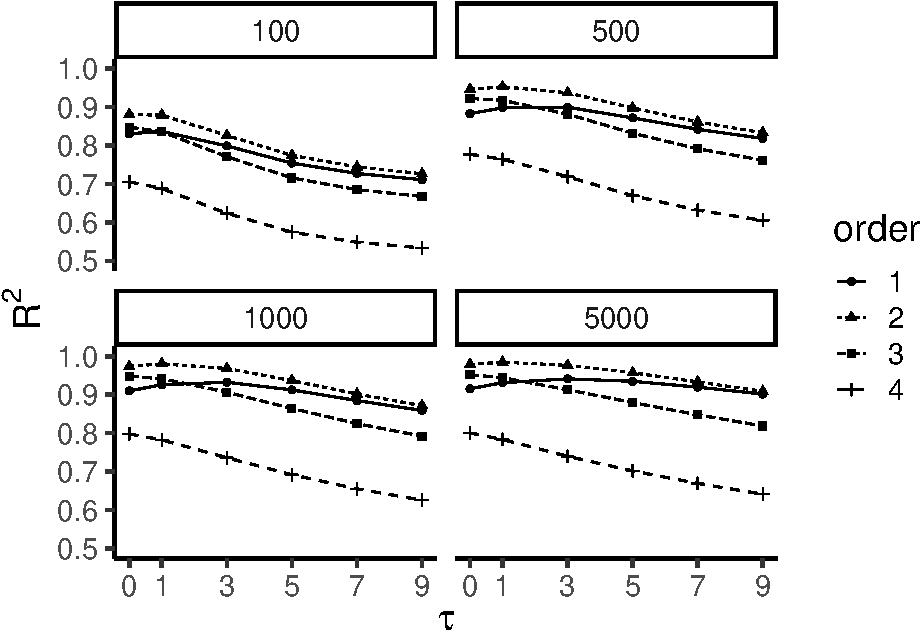
\includegraphics[width=\linewidth]{ITS_cogsci_files/figure-latex/ITSsimple-1.pdf}
\caption{\label{fig:ITSsimple}\(R^2\) values between ITS word-word similarity space, and the first to fourth order word-word similarity spaces derived the artificial language as a function of training, and retrieval gradient (tau)}
\end{figure}

ITS performed well in recovering the structure of the artificial language. Most important, ITS was most sensitive to the second-order similarity structure of the artificial language. More generally, ITS became more sensitive to all orders of similarity as training increased, and less sensitive as tau increased. Raising tau did increase relative sensitivity to the first order, but did so at the cost of losing sensitivity overall. The fact that ITS prioritizes the second order over the first is its flaw. The second order space is an overgeneralized version of the first, and blurs out the finer distinctions between word usage within the topic structures that generate the words. This is a base rate of word occurrence issue. ITS relies on second order similarity (see discussion), so semantic vectors for topic-unique words become similar to words from overlapping topics, whereas they are not similar to those words in first order space. ITS glosses over these nuances.

\subsection{Simulation 2: ITS 2 encoding}

We next trained ITS 2 with weighted expectancy subtraction at encoding on the same artificial language. We show that weighted expectancy subtraction causes ITS 2 to become more sensitive to first order word-word similarity than higher orders. In the simulations we vary the value of \(x\) (from .01 to .5) to subtract different amounts of the echo from the probe. The value of \(x\) causes systematic differences in ITS 2's sensitivity to higher order similarity structure. For clarity, we set \(tau\) to 1. The results are shown in figure \ref{fig:allsims} (left panel).

\begin{figure*}

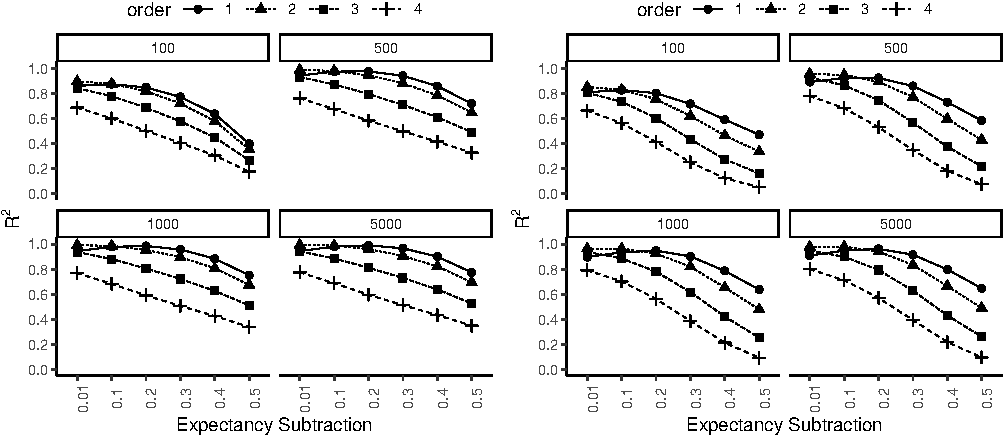
\includegraphics[width=\textwidth]{ITS_cogsci_files/figure-latex/allsims-1.pdf}

\caption{\(R^2\) values between ITS word-word similarity space and the first to fourth order word-word similarity spaces derived the artificial language as a function of training, and weighted expectancy subtraction. The left panel shows ITS 2 with weighted expectancy subtraction during encoding, and the the right panel shows ITS 2 with weighted expectancy subtraction during retrieval.}\label{fig:allsims}
\end{figure*}

% \begin{figure}
% \centering
% 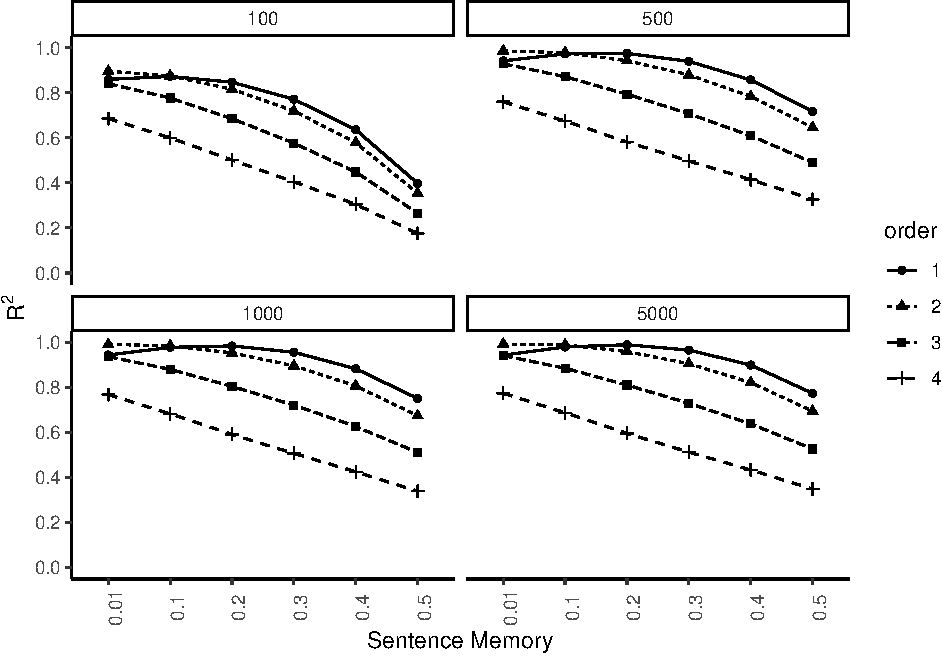
\includegraphics[width=\linewidth]{ITS_cogsci_files/figure-latex/ITSencodinglinear-1.pdf}
% \caption{\label{fig:ITSencodinglinear}\(R^2\) values between simple ITS word-word similarity space, and the first to fourth order word-word similarity spaces derived from the artificial language as a function of training, and weighted expectancy subtraction at encoding. The retrieval gradient (tau) was set to 1.}
% \end{figure}

Weighted expectancy subtraction at encoding modulated how ITS 2 recovered different orders of semantic similarity space. For example, when \(x=.01\), ITS 2 was most sensitive to second order similarity, but as \(x\) increased ITS 2 became most sensitive to first-order similarity. Increasing \(x\) further caused overall sensitivity to decline \cite<akin to the detrimental effects of sub-sampling too much negative information, >{johnsRoleNegativeInformation2019}. It appears that ITS 2 is capable of recovering more veridical and nuanced word embeddings from the first-order similarity space.

\subsection{Simulation 3: ITS 2 retrieval}

Here, we trained ITS 2 with weighted expectancy subtraction at retrieval only. We repeated the above simulation exactly, but used the equations involving one iterative retrieval step to conduct the weighted expectancy subtraction at retrieval. We also used a \(tau\) of 0 to compute both echoes, or a square retrieval gradient. We chose this value to foreshadow a correspondence between transformations of the defined artificial language in higher order similarity space, and what ITS 2 is achieving at retrieval by subtracting a portion of the second echo from the first. The results are shown in figure \ref{fig:allsims} (right panel).

% \begin{figure}
% \centering
% 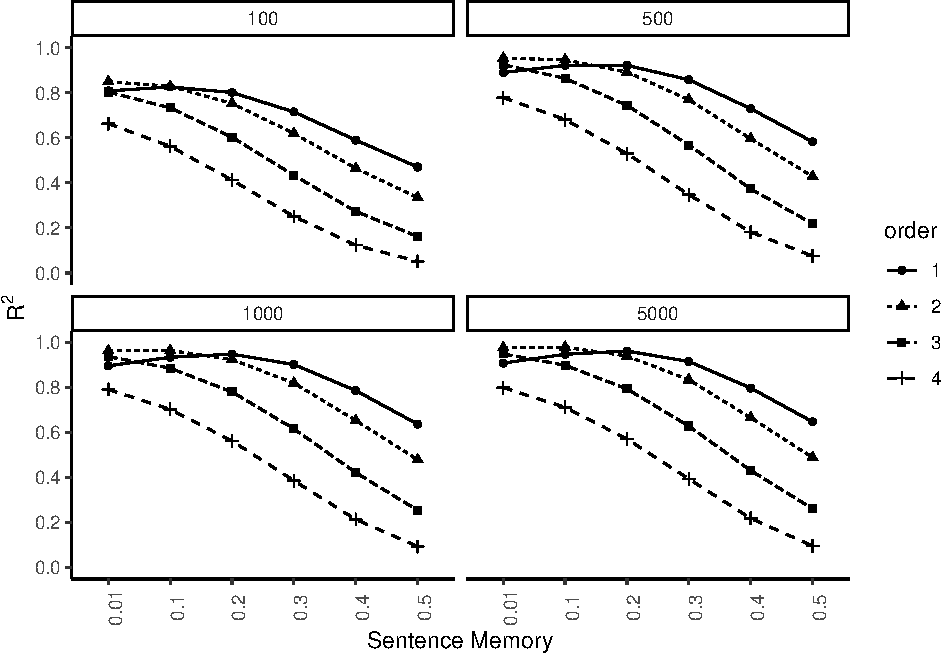
\includegraphics[width=\linewidth]{ITS_cogsci_files/figure-latex/ITSretrieval-1.pdf}
% \caption{\label{fig:ITSretrieval}\(R^2\) values between simple ITS word-word similarity space, and the first to fourth order word-word similarity spaces derived from the artificial language as a function of training, and weighted expectancy subtraction at retrieval.}
% \end{figure}

Remarkably, ITS 2 does not need to make any assumptions about encoding to benefit from weighted expectancy subtraction. The pattern of Simulation 3 is almost identical to that of Simulation 2. Specifically, ITS 2 becomes most sensitive to first-order word-word similarity structure as \(x\) is increased. Again, increasing \(x\) has diminishing returns.

\section{General Discussion}

Distributional models of semantic cognition become sensitive to co-occurrence structure in natural text. By defining analogous sources of co-occurrence structure in an artificial language, we determined the aspects of that structure recovered by ITS and ITS 2. We showed that ITS is most sensitive to second order semantic space. We also showed that ITS 2 can modulate its sensitivity by a process of weighted expectancy subtraction and iterative retrieval. Impressively, these operations allowed ITS 2 to become most sensitive to first order semantic space, which is a more veridical representation by our definition.

It is instructive to consider how ITS and ITS 2 recover different orders of similarity space. First, consider how words become increasingly similar across orders of similarity space. In the first order, word similarity is determined by the topics they occur in. For example, word 6 is only similar to topic one words, and word 15 is similar to topic one and two words because it occurs in both topics. In the second order, words become similar on the basis of their first order similarity features. First order features for word 6 now contain positive similarity for words 1 to 15 (all topic one). Some of these features are shared by words from topic two. As a result, words unique to topic one become similar to words from neighboring topics. If there is a series of partial overlap connecting words across topics, then all words become increasingly similar to all words across increasing orders of similarity, and the nth order similarity matrix becomes all ones.

Crucially, iterative retrieval in ITS 2 is a process for traversing higher-order similarity space; and weighted expectancy subtraction is a process for negotiating the the relative contributions of higher-order similarity representations in the construction of semantic knowledge. To elaborate, we showed that ITS echoes are most sensitive to the second order. Echoes contain sentence memory, so an echo for a topic-unique word contains words that overlap in neighboring topics. Thus, semantic vectors for topic-unique words become similar to words from neighboring topics. Submitting the echo as a probe for iterative retrieval is a third order operation. The echo contains many words and the second echo collapses over memory for sentences that contain any of those words. This draws in sentences from additional topics, causing a given word to be more similar to words in outlying topic neighborhoods. Iterating to the extreme sweeps all sentences in memory into the echo, causing identical echoes for all words.

Simulation 3 showed that subtracting a portion of the second echo from the first allows ITS 2 to preferentially recover first order similarity space. Our preceding discussion suggests ITS 2 performs a weighted subtraction of third from second order space, suggesting a similar result could be obtained analytically. We confirmed this directly from the language by subtracting proportions of the third order similarity matrix from the second, and computing \(R^2\) between each new matrix and the first order similarity matrix. We found an inverse U function, with \(R^2\) approaching 1 at .4. As a side-note, computing second order similarity from a document term matrix  \cite{cribbinDiscoveringLatentTopical2011} can produce embeddings similar if not superior to those produced by singular value decomposition, as in LSA. We speculate that subtracting a portion of the third order from the second may further improve the quality of those semantic representations.

In the future we plan to apply ITS and ITS 2 to natural language and compare the quality of word-embedding by fits to human performance in semantic tasks. At present we offer ITS 2 as an intriguing account of how people may transform their semantic knowledge along general versus specific lines, by using iterative memory retrieval to traverse higher order similarity space, and weighted expectancy subtraction to control the specificity of retrieved semantic knowledge.

%
%
% Using the identity matrix to represent words, and setting tau to 0, ITS memory becomes a simple document-term matrix, and the echo for any probe is the sum of document vectors that contain the probe word. Consider that in first order space, words that are unique to one topic (e.g., words 6-10 for topic one) are only similar to themselves, and have zero similarity to all other words. However, this changes in second order space.
%
% If we use an identity matrix to represent words, and set tau to 0, it becomes
%
% It is not surprising that ITS is most sensitive to second order similarity space. Co
%
% We now attempt to clarify analytic relationships between ITS semantic vectors and higher order similarity space
%
%
% Our simulation approach offered some insight into
%
% We have shown that simple ITS is most sensitive to the second order word-word similarity structure of the artificial language. We discussed how iterative retrieval produces echoes that would become more sensitive to increasing orders of word-word similarity space. Simulation 3 showed that subtracting a portion of the second echo from the first cause ITS 2 to become more sensitive to first order word-word similarity. These relationship suggest that weighted expectancy subtraction is a transform that can be applied directly to higher order similarity space, if that space is known.
%
% In our case, the nth-order word-word similarity space is completely determined by the topic-word probability matrix of the artificial language. As a result, we can determine whether subtraction of a higher-order similarity space from a lower order similarity produces similar results. We assume that ITS 2 is performing an operation similar to subtracting a proportion of third-order word-word similarity space from it's representation of second-order word-word similarity space, and this subtraction results in an echo most sensitive to first-order word-word similarity space. We now show this by subtracting weighted portions of third-order word-word similarity space from the second-order to arrive at the first-order, directly from the basis functions of the artificial language.



% \section{Acknowledgments}
%
% In the \textbf{initial submission}, please \textbf{do not include
%   acknowledgements}, to preserve anonymity.  In the \textbf{final submission},
% place acknowledgments (including funding information) in a section \textbf{at
% the end of the paper}.

\bibliographystyle{apacite}

\setlength{\bibleftmargin}{.125in}
\setlength{\bibindent}{-\bibleftmargin}

\bibliography{ITS}


\end{document}
